% activity 1.1
\subsection{Sinusoidal reference generation}
The objective of this activity is display the UR5 robot on rviz. The simulation should start with the   initial joint configuration $\begin{bmatrix} \pi & -\frac{\pi}{8} & -\frac{\pi}{6} & 0.0 & 0.0 & 0.0 \end{bmatrix}$ and then move the second and fifth joint. The joints will move with a sinusoidal reference during the first 4 seconds and maintain a constant joint position during the last second. The function to generate the sinusoidal reference is describe in Algorithm \ref{lst:sine_reference_generator} and the rosnode file to move the second and fifth joint of UR5 robot is describe in Algorithm \ref{lst:rosnode_sine_reference_generator}. Finally, Figure \ref{fig:act1.1_joint_position}-\ref{fig:act1.1_joint_acceleration} shows the joint position, velocity and acceleration of each joint of the UR5 robot.

\begin{lstlisting}[language=Python,caption=Function to generate sinusoidal reference., label={lst:sine_reference_generator}]
    def sinusoidal_reference_generator(q0, dq0, ddq0, a, f, t):
    """
    Info: generates a sine signal.

    Inputs: 
    ------
        - q0: initial joint position
        - dq0: initial joint velocity
        - ddq0: initial joint acceleration
        - a: amplitude [rad]
        - f: frecuency [hz]
        - t: simulation time [sec]
    Outputs:
    -------
        - sinusoidal signal
    """
    w = 2*np.pi*f               # [rad/s]
    q = q0 + a*np.sin(w*t)           # [rad]
    dq = dq0 + a*w*np.cos(w*t)        # [rad/s]
    ddq = ddq0 -a*w*w*np.sin(w*t)    # [rad/s^2]

    return q, dq, ddq
\end{lstlisting}
%Rosnode to move the second and fifth joint of UR5 robot. On one hand, the second joint will follow the sinusoidal reference $0.2\sin{2\pi t}$ during the first $4$ seconds and maintain a constant angular position during the last second. On the other hand, the fifth joint will follow the sinusoidal reference $0.4\sin{3\pi t}$ during the first $4$ seconds and maintain a constant angular position during the last second.
\begin{lstlisting}[language=Python,caption={Rosnode to move the second and fifth joint of UR5 robot with the requirement motion of activity 1.1.} ,label={ lst:rosnode_sine_reference_generator}]
    # =========================
    #   Configuration of node
    # =========================
    # create a node: 
    rospy.init_node("node_sinusoidal_reference_generation")
    
    # public in topic /joint_states	to send joint data	
    pub = rospy.Publisher('joint_states', JointState, queue_size=1000)
    
    # loop rate (in Hz)
    rate 	= rospy.Rate(1000)		# [Hz]
    dt 		= 1e-3					# [ms]
    
    # object(message) type JointState
    jstate = JointState()
    
    # ===========================
    #   UR5 robot configuration
    # ===========================
    # joints name of UR5 robot
    jnames = ['shoulder_pan_joint', 'shoulder_lift_joint', 'elbow_joint','wrist_1_joint', 'wrist_2_joint', 'wrist_3_joint']
    # number of degress of freedom
    ndof = 6
    
    # ==========================================
    #   Set initial joint configuration of UR5
    # ==========================================
    # initial configuration: position, velocity and acceleration 
    q0   = np.array([np.pi, -np.pi/8,  -np.pi/6, 0.0, 0.0, 0.0])
    dq0  = np.array([0.0, 0.0, 0.0, 0.0, 0.0, 0.0])
    ddq0 = np.array([0.0, 0.0, 0.0, 0.0, 0.0, 0.0]) 
    
    # desired trajectory: position, velocity and acceleration
    q_des   = np.zeros(ndof)
    dq_des  = np.zeros(ndof)
    ddq_des = np.zeros(ndof)
    
    #===============
    #   Simulation
    #===============
    t = 0.0             # [sec] 
    sim_duration = 5.0  # [sec]
    sine_duration = 4.0 # [sec]
    
    while not rospy.is_shutdown():
        # generate sine or step joint reference
        if t<=sine_duration:
            # second link
            q_des[1], dq_des[1], ddq_des[1] = sinusoidal_reference_generator(q0[1], dq0[1], ddq0[1], 0.2, 1, t)
            # fifth link
            q_des[4], dq_des[4], ddq_des[4] = sinusoidal_reference_generator(q0[4], dq0[4], ddq0[4], 0.4, 1.5, t)
    
        # publish message
        jstate.header.stamp = rospy.Time.now()
        jstate.name 		= jnames    # Joints position name
        jstate.position 	= q_des     # joint position
        jstate.velocity 	= dq_des    # joint velocity
        pub.publish(jstate)
    
        # update time
        t = t + dt

        # stop simulation
        if t>=sim_duration:
            print("stopping rviz ...")
            break  
        rate.sleep()
\end{lstlisting}


\begin{figure}
    \centering
    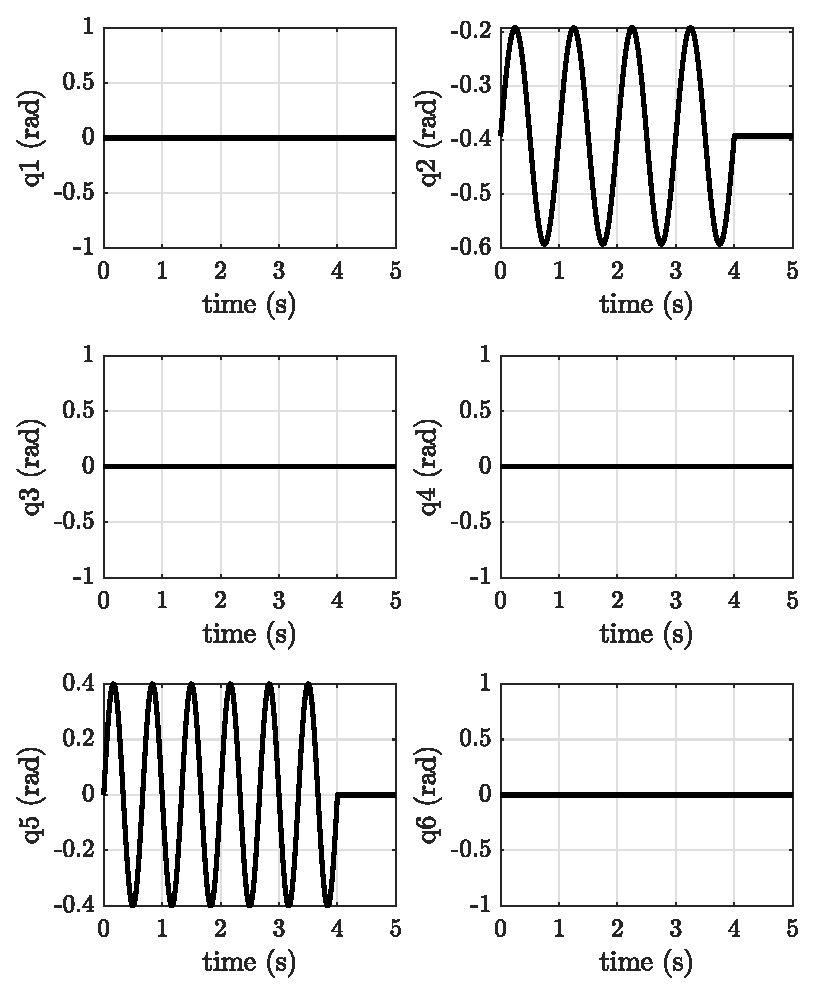
\includegraphics{images/act_1.1/joint_position.eps}
    \caption{Angular position of each joint of UR5 robot with Algorithm \ref{lst:rosnode_sine_reference_generator}.}
    \label{fig:act_1.1_joint_position}
\end{figure}

\begin{figure}
    \centering
    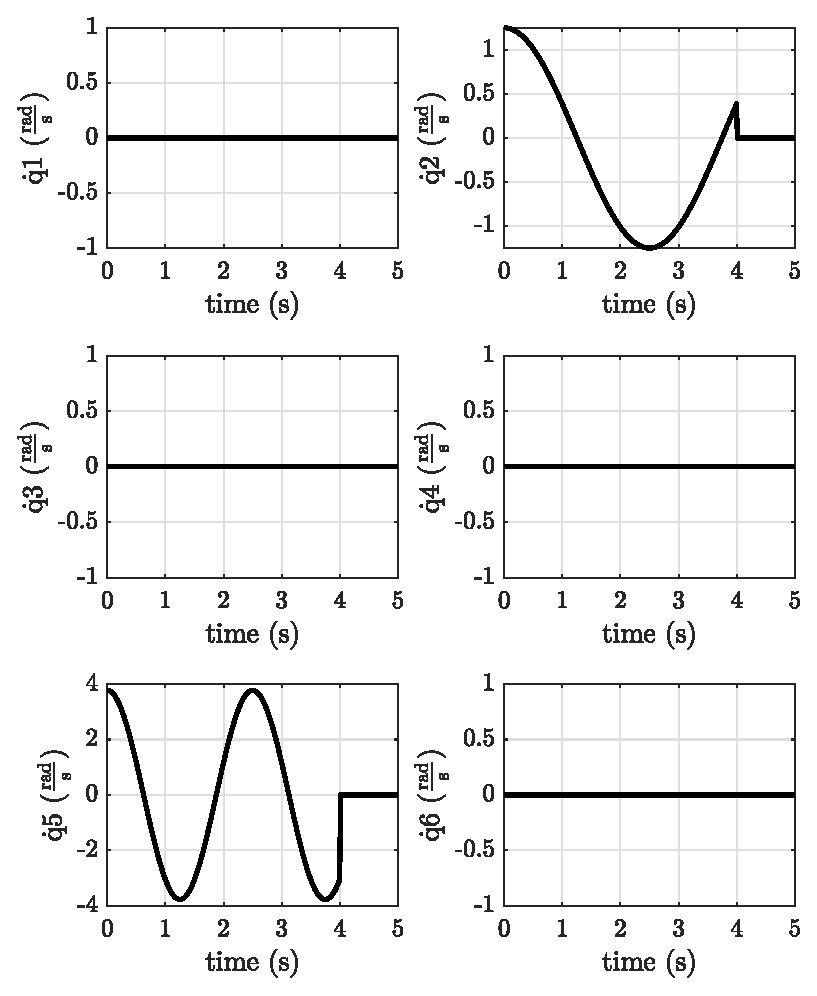
\includegraphics{images/act_1.1/joint_velocity.eps}
    \caption{Angular velocity of each joint of UR5 robot with Algorithm \ref{lst:rosnode_sine_reference_generator}.}
    \label{fig:act_1.1_joint_velocity}
\end{figure}

\begin{figure}
    \centering
    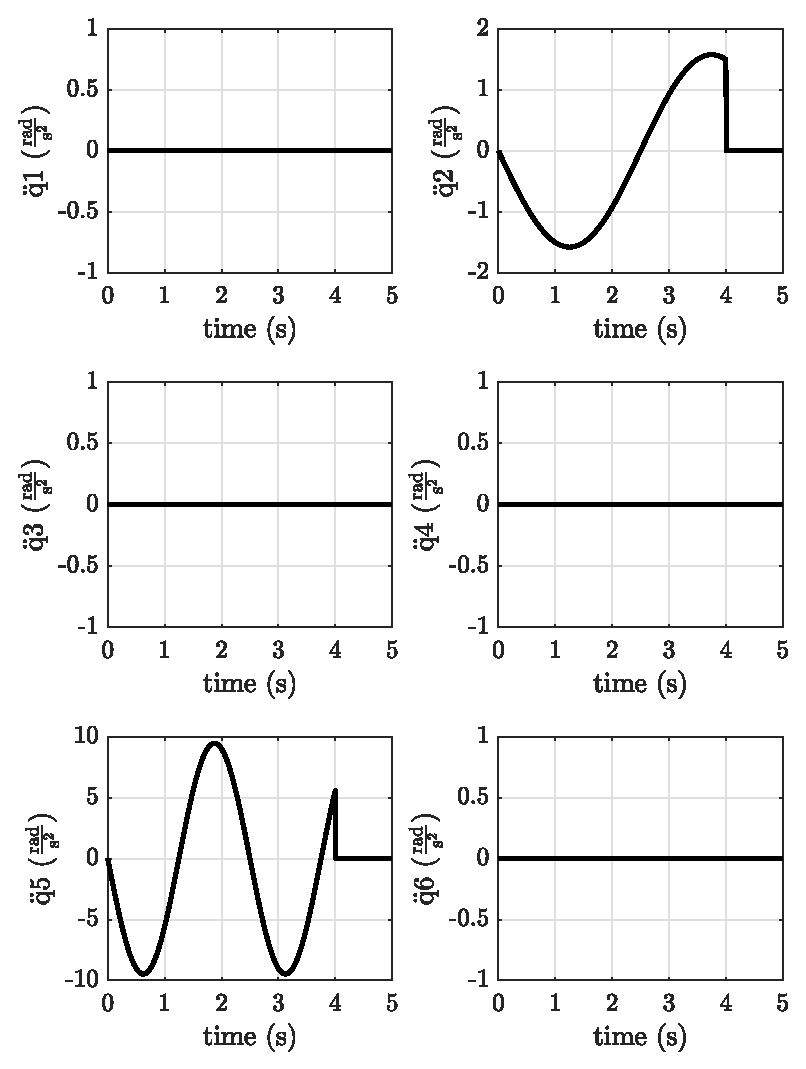
\includegraphics{images/act_1.1/joint_acceleration.eps}
    \caption{Angular acceleration of each joint of UR5 robot with Algorithm \ref{lst:rosnode_sine_reference_generator}.}
    \label{fig:act_1.1_joint_acceleration}
\end{figure}